\section{Quantitative Comparison}
Here goes the quantitative comparison.

\subsection{Experiment Setup}
The different setups of the experiments are all based on the IoTivity framework running on two Linux (Ubuntu) machines. These two machines are both wireless coupled to a local network via a router. The test case for the experiments is meant to represent a constrained device, acting as a client, updating the temperature on a cloud server with a specific interval of time. 

Linux is chosen to represent a constrained device as it is necessary to be able to easily monitor the communication from the client side of view.

Setup for CoAP over UDP as illustrated in \figurename \ref{fig:setupudp} uses two applications. A simple IoTivity client and server application both developed in C++ using CoAP over UDP as an application protocol.
\begin{figure}[!t]
	\centering
	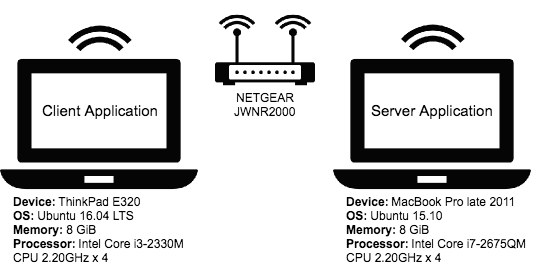
\includegraphics[width=3in]{gfx/setupa}
	\caption{Setup for CoAP over UDP.}
	\label{fig:setupudp}
\end{figure}

Setup for CoAP over TCP as illustrated in \figurename \ref{fig:setuptcp} uses two applications. A simple IoTivity client application developed in C++ and a simple IoTivity server application developed in Java. Both applications uses CoAP over TCP as an application protocol.
\begin{figure}[!t]
	\centering
	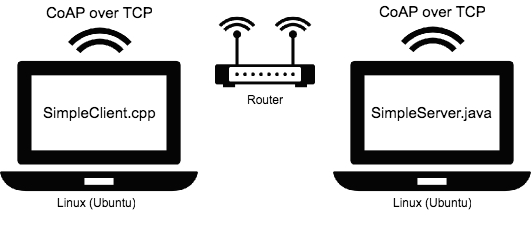
\includegraphics[width=3in]{gfx/setupb}
	\caption{Setup for CoAP over TCP.}
	\label{fig:setuptcp}
\end{figure}

The memory consumption for the two client applications is presented in table \ref{tab:memory}:
%TABLE
The RAM measurements are done by using an AVR-tool called avr-size. The tool measures only the size of the initialized variables.
%Wireshark....
%\textbf{Memory consumption}\\
%Flyt den del til et afsnit med prototype implementation (før resultaterne)
%How much memory usage...

\subsection{Bandwidth}
In the following experiments the bandwidth of a \emph{single packet transaction} and the bandwidth of a \emph{complete communication scenario} for both aforementioned setups are measured. 
Bandwidth generated by communication protocols is directly related to the energy consumption. By measuring the bandwidth in bytes and multiplying it with the energy consumption of sending a single byte using Arduino Due, it is possible to calculate the complete energy consumption of the used constrained devices. 

\subsubsection{Single Packet Transaction}
This experiment is done where the client transmits a single packet, containing an arbitrary number, simulating a temperature measurement. \figurename{\ref{fig:singlepacket}} shows the results for a single packet transaction scenario, where CoAP (NON) and CoAP (CON) are the two different modes for CoAP over UDP. %CoAP (NON) is non-confirmable which means that the
\begin{figure}
	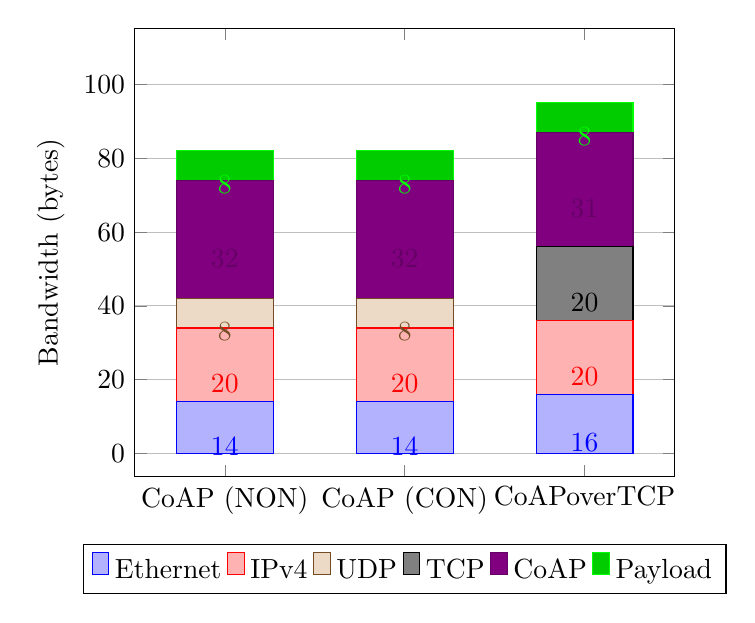
\begin{tikzpicture}
	\begin{axis}[
	%title={Single Packet Transaction (Client/Server)},
	ybar stacked,
	%ymax=50,
	ymajorgrids,
	bar width=35pt,
	%width=250pt,
	nodes near coords, 
	%nodes near coords={\pgfmathprintnumber\pgfplotspointmeta \%},
	nodes near coords align={anchor=north},%Move values in bar
	every node near coord/.style={
	},
	enlargelimits=0.25,
	legend style={at={(0.5,-0.15)},
		anchor=north,legend columns=-1},
	%width=0.8*\textwidth,
	ylabel={Bandwidth (bytes)},
	symbolic x coords={CoAP (NON), CoAP (CON), CoAPoverTCP},
	xtick=data,
	%legend pos= north east,
	%x tick label style={rotate=45,anchor=east},
	]
	%ethernet
	\addplot+[ybar] plot coordinates {(CoAP (NON),14) (CoAP (CON),14)
		(CoAPoverTCP,16) };
	%ipv4
	\addplot+[ybar] plot coordinates {(CoAP (NON),20) (CoAP (CON),20) 
		(CoAPoverTCP,20) };
	%udp
	\addplot+[ybar] plot coordinates {(CoAP (NON),8) (CoAP (CON),8) 
		(CoAPoverTCP,0) };
	%tcp
	\addplot+[ybar] plot coordinates {(CoAP (NON),0) (CoAP (CON),0) 
		(CoAPoverTCP,20) };
	%coap 
	\addplot+[ybar] plot coordinates {(CoAP (NON),32) (CoAP (CON),32) 
		(CoAPoverTCP,31) };
	%payload
	\addplot+[ybar] plot coordinates {(CoAP (NON),8) (CoAP (CON),8) 
		(CoAPoverTCP,8) };
	
	\legend{\strut Ethernet, \strut IPv4, \strut UDP, \strut TCP , \strut CoAP, \strut Payload}
	\end{axis}
	\end{tikzpicture}
	\caption{Single Packet Transaction (Client/Server).}
	\label{fig:singlepacket}
\end{figure}
It can be observed that CoAP over TCP overall has a lager packet than CoAP over UDP. This is primarily because of the TCP layer which has a 12 byte bigger overhead than UDP.
Though the CoAP layer in the CoAP over TCP packet is 1 byte shorter than CoAP over UDP, because of the MessageID-field (2 byte) is removed and replaced with the Length-field (1 byte).
%Why is ethernet 16 bytes???

With help of the measurements the energy consumption is calculated for the three packets. The calculation is shown below:
%calculation...

%TCP minimum header size is 20 bytes, but because of using options among others timestamp option, it is measured to 32 bytes. Timestamp option is enabled par default on Ubuntu 16.10.

\subsubsection{Complete Communication Scenario}
This experiment is done where the client transmits randomly generated numbers with an interval of 30 seconds, simulating temperature measurements, for a timespan of 30 minutes.
It is a complete scenario because the whole communication scenario, from it is initialised until it is terminated, is captured. The caption includes both the transmitted and the received packets.

\figurename{\ref{fig:completescenario}} shows the results for a complete scenario, where CoAP (NON) is omitted as it is not comparable with the two reliable CoAP versions, CoAP (CON) and CoAP over TCP. 
\begin{figure}[bht]
	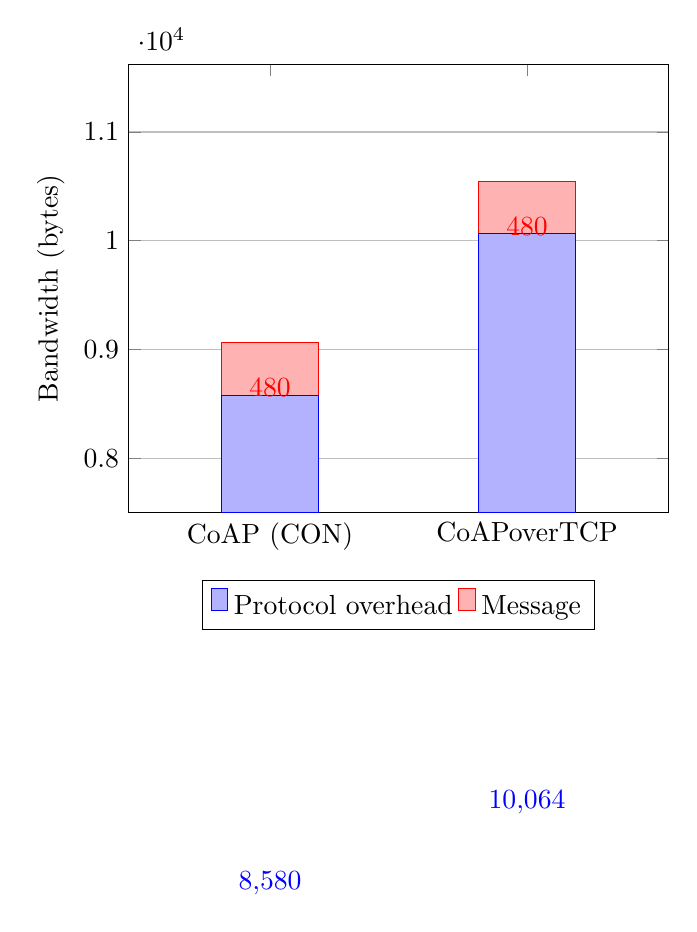
\begin{tikzpicture}
	\begin{axis}[
	%title={A complete communication scenario},
	ybar stacked,
	%ymax=50,
	ymajorgrids,
	bar width=35pt,
	%width=250pt,
	nodes near coords, 
	%nodes near coords={\pgfmathprintnumber\pgfplotspointmeta \%},
	nodes near coords align={anchor=north},%Move values in bar
	every node near coord/.style={
	},
	enlargelimits=0.55,
	legend style={at={(0.5,-0.15)},
		anchor=north,legend columns=-1},
	%width=0.8*\textwidth,
	ylabel={Bandwidth (bytes)},
	symbolic x coords={CoAP (CON), CoAPoverTCP},
	xtick=data,
	%legend pos= north east,
	%x tick label style={rotate=45,anchor=east},
	]
	%protocol overhead
	\addplot+[ybar] plot coordinates { (CoAP (CON),8580) 
		(CoAPoverTCP,10064) };
	%message
	\addplot+[ybar] plot coordinates { (CoAP (CON),480) 
		(CoAPoverTCP,480) };
	
	\legend{\strut Protocol overhead, \strut Message}
	\end{axis}
	\end{tikzpicture}
	\caption{A complete communication scenario.}
	\label{fig:completescenario}
\end{figure}

It is clear from the results that CoAP over TCP has a significantly larger overhead than CoAP (CON).
 
With help of the measurements the energy consumption is calculated for the two scenarios. The calculation is shown below:
%calculation...
%\textbf{En god ide er at maale energiforbruge / beregne det i joule. Giver et konkret svar om den kan bruges i specifikke typer af constraint devices}

\subsection{Latency}
In the following experiments the latency (RTT) is measured for the two setups in two scenarios, one with a noiseless channel and the other with a simulated noisy channel. The latency has an impact on the energy consumption. A long latency means less sleeping time which is a crucial element for a constrained to be able to save energy.
The noisy channel is emulated using the NetEM tool which provides Network Emulation functionality for testing protocols \cite{netem19:online}. 

These experiments are all done where the client transmits a total number of 60 transmissions. The RTT is calculated from the time a packet is sent until it receives the associated acknowledgement.

%Measure RTT values %which is the time from sending a package to receiving the acknowledgement.
%More latency = less time to sleep = more energy consumption
%Spredning/fordeling/varians af delay variations 

On \figurename{\ref{fig:coapconlatency}} and \figurename{\ref{fig:coaptcplatency}} the results of the first scenario with a noiseless channel for the respectively CoAP over UDP and CoAP over TCP setup are plotted into a histogram. 
\begin{figure}[bht]
	\centering
	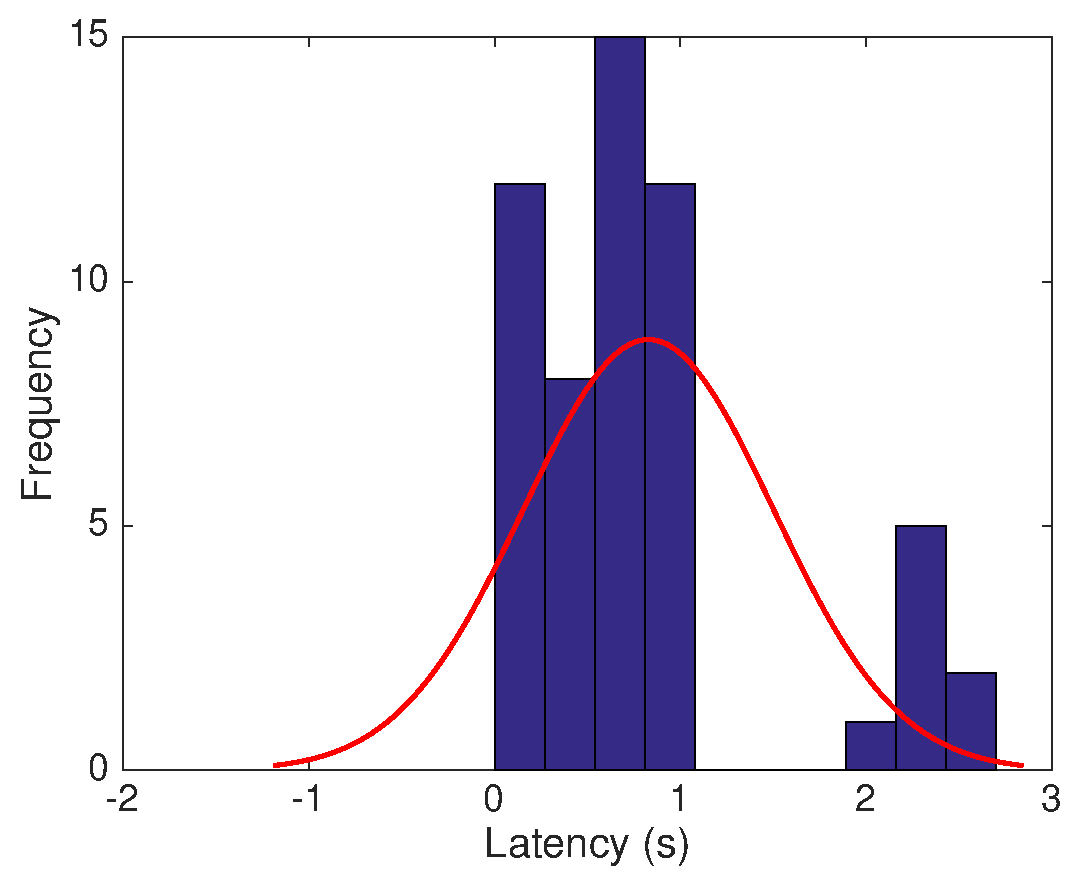
\includegraphics[width=3in]{gfx/coapoverudp}
	\caption{Latency for CoAP over UDP in a noiseless channel.}
	\label{fig:coapconlatency}
\end{figure}
\begin{figure}[bht]
	\centering
	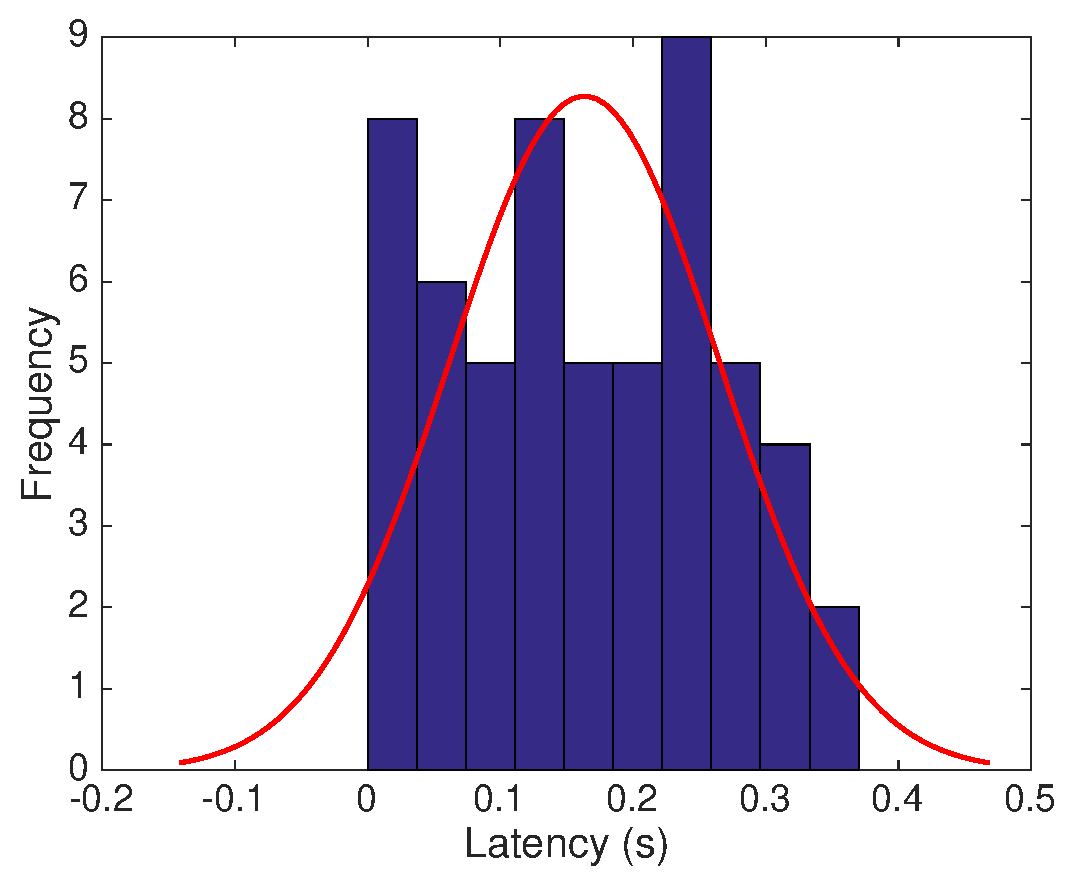
\includegraphics[width=3in]{gfx/coapovertcp}
	\caption{Latency for CoAP over TCP in a noiseless channel.}
	\label{fig:coaptcplatency}
\end{figure}

From the results it is observed  that the latency varies from 0 seconds up to 3 seconds for CoAP over UDP and from 0 seconds up to 0.4 seconds for CoAP over TCP. Thereby it is clear that CoAP over TCP has a faster round trip than CoAP over UDP. 

%TCP direct from transport layer therefore faster
%UDP from application layer therefore slower


%More lost packet = more packet to send = more energy consumption
This is the \figurename \ref{coapovertcploss}
\begin{figure}[bh]
	\centering
	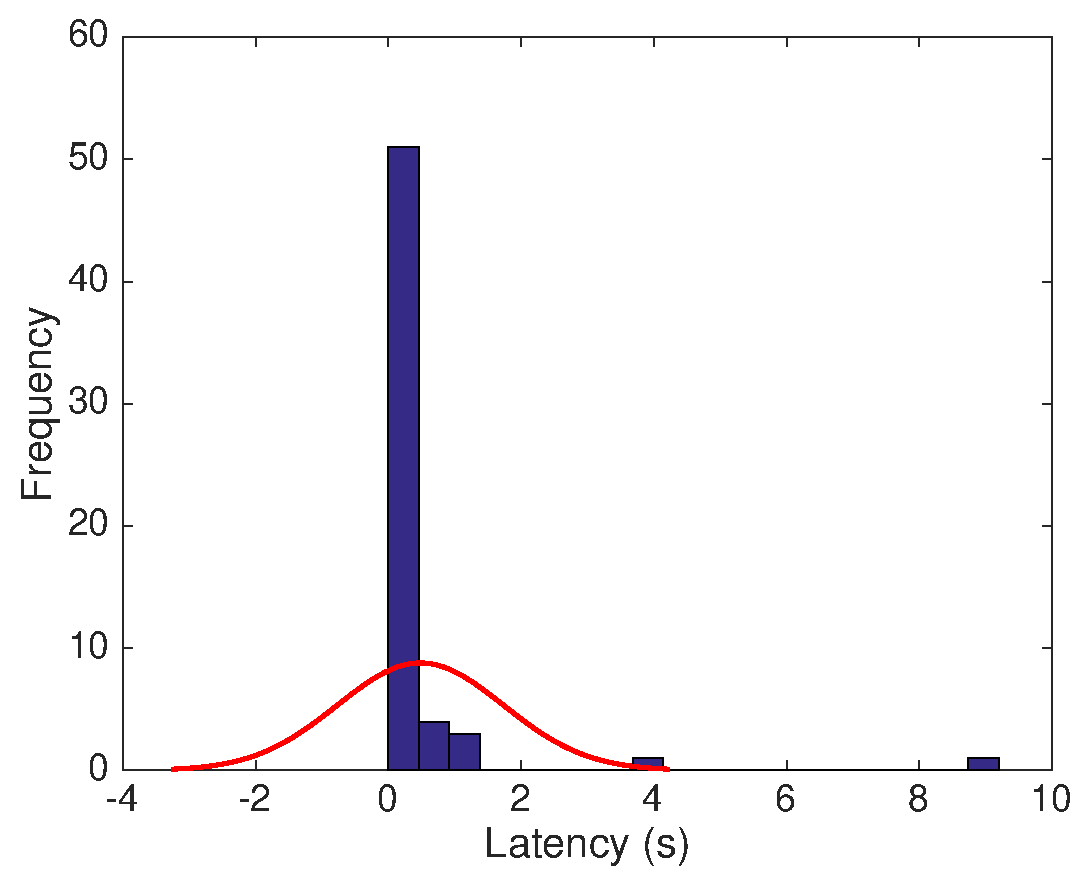
\includegraphics[width=3in]{gfx/coapovertcp25loss}
	\caption{Latency for CoAP over TCP with 25 \% packet loss.}
	\label{coapovertcploss}
\end{figure}

This is the \figurename \ref{coapoverudploss}
\begin{figure}[bh]
	\centering
	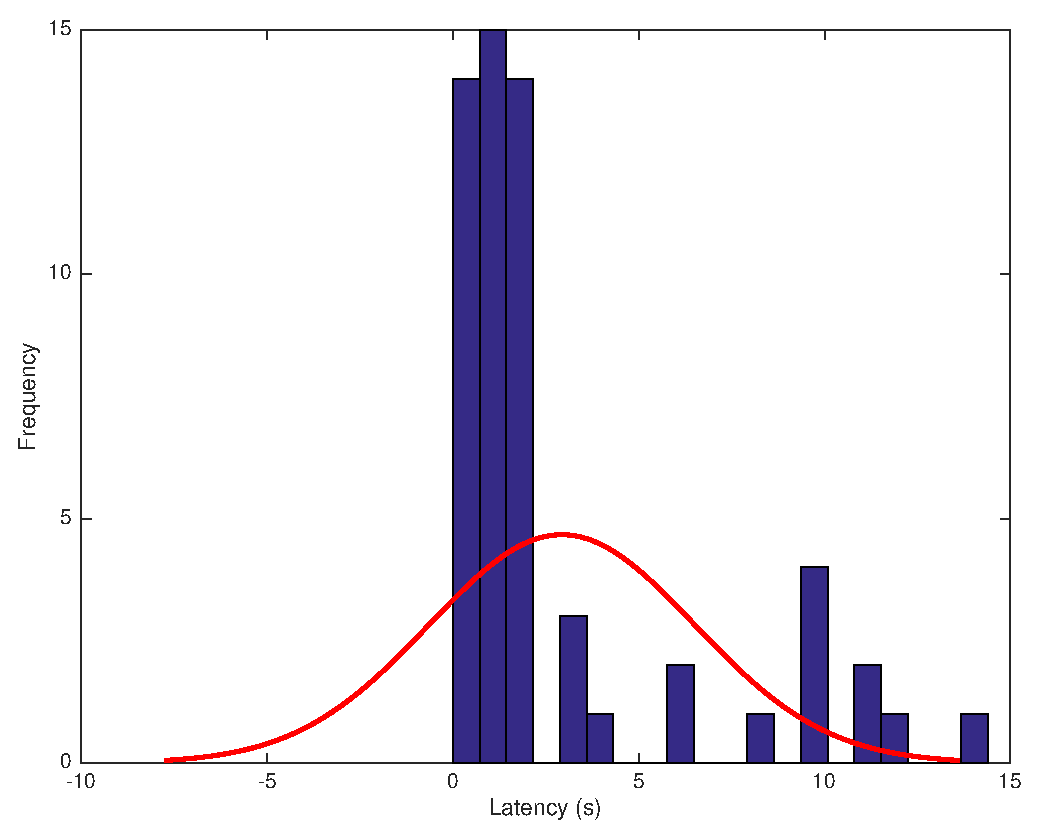
\includegraphics[width=3in]{gfx/coapoverudp25loss}
	\caption{Latency for CON CoAP with 25 \% packet loss.}
	\label{coapoverudploss}
\end{figure}

